% iden3. Pedersen specification.
% Marta Belles. Jan-Feb 2019.

\documentclass{article} 

\usepackage[ colorlinks=true,
			 urlcolor=black,
			 linkcolor=black,
			 citecolor=black
			]{hyperref} 
		
\usepackage[english]{babel}
\usepackage[utf8]{inputenc}
\usepackage{amsmath, amsthm, amssymb}
\usepackage{enumerate, enumitem}
\usepackage{graphicx}
\usepackage{color, xcolor}
\usepackage{setspace}
\usepackage{hyperref}

\textwidth 16 cm
\textheight 22 cm
\topmargin -1 cm
\oddsidemargin -0 cm

\addtolength{\skip\footins}{1pc plus 5pt} % Foot note space
\setlength\parindent{0pt} % No indent

\newcommand{\noi}{\noindent}

\newcommand{\N}{\ensuremath{\mathbb{N}}}
\newcommand{\Np}{\ensuremath{\mathbb{N}^{+}}}
\newcommand{\Z}{\ensuremath{\mathbb{Z}}}
\newcommand{\Q}{\ensuremath{\mathbb{Q}}}
\newcommand{\R}{\ensuremath{\mathbb{R}}}
\newcommand{\C}{\ensuremath{\mathbb{C}}}
\newcommand{\Fp}{\ensuremath{\mathbb{F}_p}}
\newcommand{\G}{\ensuremath{\mathbb{G}}}
\newcommand{\maxBits}{200}
\newcommand{\point}[1]{P_{#1} = (x_{#1}, y_{#1})}
\newcommand{\gen}[1]{\ensuremath{\langle #1\rangle}}



\title{%
	Pedersen hash specification 
	\vspace{-0.2cm} 
	}
\author{
\includegraphics[scale=0.3]{iden3.png}}

\begin{document}
\begin{spacing}{1.2}

\maketitle
\vspace{1cm}
\tableofcontents

\vspace{0.5cm}

\newpage
\section{Elliptic curve: Baby-Jubjub}			Let $p$ be a prime number and $\Fp$ the finite field with $p$ elements. Let $E$ be an elliptic curve defined over $\Fp$ of order $n = h\times r$, where $r$ is a large prime and $h$ is typically a small positive integer called cofactor.\\ 
% The notation used in this document is the following one.

\begin{table}[htp]
	\begin{center}
	\begin{tabular}{c|c|c}
		{\bf Group} & {\bf Description} & {\bf Order} \\
		\hline 
		$\Fp$ & Finite field with $p$ elements & $p$\\
		$E$ & Elliptic curve group & $n = h\times r$\\
		$\G \subseteq E$ & Subgroup of points of $E$ of order $r$ & $r$%\\
	\end{tabular}
	\end{center}
\end{table}
	\subsection{Twisted Edwards form}			We define the twisted Edwards curve {\it Baby-Jubjub} defined over $\Fp$ with 
	$$	p = 21888242871839275222246405745257275088548364
			400416034343698204186575808495617 $$
described by 
	$$	E: 168700 x^2 + y^2 = 1 + 168696 x^2 y^2. $$  

The order of $E$ is $8\times r$, where 
	$$	r = 2736030358979909402780800718157159386076813
			972158567259200215660948447373041. $$ 
The rest of specifications and the satisfiability of SafeCurves criteria  of this curve can be found in \cite{github-barry}. 
	\subsection{Montgomery form}				{\it{Baby-Jubjub}} is birationally equivalent to the Montgomery elliptic curve defined by  
	$$ E_M : v^2 = u^3 + 168698 u^2 + u. $$
The birational equivalence from $E$ to $E_M$ is the map 
	$$ (x,y) \to (u,v) = \left( \frac{1 + y}{1 - y} , \frac{1 + y}{(1 - y)x} \right) $$
with inverse from $E_M$ to $E$
	$$ (u, v) \to (x, y) = \left(  \frac{u}{v}, \frac{u - 1}{u + 1}   \right). $$
These results are from \cite[Theorem 3.2]{twisted}.

\section{Arithmetic on the elliptic curve}		In this section we define two operations supported in the elliptic curve group: addition of points and multiplication of a point by a scalar (an element of $\Fp$).

	\subsection{Addition of points}				When adding points of elliptic curves %usually
in Montgomery form,  
one has to be careful if the points being added are equal (doubling) or not (adding) and if one of the points is the point at infinity \cite{montgomery}. 
%
Twisted Edwards curves have the advantage that there is no such case distinction and doubling can be performed with exactly the same formula as addition \cite{twisted}. 
%
In comparison, operating in Montgomery curves is cheaper. In this section, we summarize how addition and doubling is performed in both forms. 
%
For the exact number of operations required in different forms of elliptic curves, see \cite{operations-cost}.

\begin{itemize}
	
	\item \underline{Twisted Edwards}: 	
	% https://eprint.iacr.org/2008/013.pdf (sec 6)
	Let $\point{1}$ and $\point{2}$ be points of the Baby-Jubjub twisted Edwards elliptic curve $E$. The sum $P_1 + P_2$ is a third point $P_3 = (x_3, y_3)$ with 
		\begin{align*}
			&\lambda = 168696 x_1x_2y_1y_2,\\
			&x_3 = (x_1y_2 + y_1x_2) / (1 + \lambda),\\
			&y_3 = (y_1y_2 - 168700 x_1x_2) / (1 - \lambda).
		\end{align*}
	Note that the neutral element is the point $O = (0,1)$ and the inverse of a point $(x,y)$ is $(-x,y)$.

	\item \underline{Montgomery}: 
	% https://link.springer.com/content/pdf/10.1007/978-3-540-46588-1_17.pdf
	Let $\point{1}\not=O$ and $\point{2}\not=O$ be two points of the Baby-JubJub elliptic curve $E_M$ in Montgomery form. 
	
	If $P_1\not=P_2$, then the sum $P_1 + P_2$ is a third point $P_3 = (x_3, y_3)$ with coordinates
	% Addition
		\begin{align}
		\label{eq-ted}
		\begin{split}
			&\Lambda = (y_2-y_1)/ (x_2-x_1),\\
			&x_3 = \Lambda^2 - 168698 - x_1 - x_2,\\
			&y_3 = \Lambda(x_1- x_3) - y_1.
		\end{split}
		\end{align}
	%
	If $P_1 = P_2$, then $2\cdot P_1$ is a point $P_3 = (x_3, y_3)$ with coordinates
	% Doubling:
		\begin{align}
		\label{eq-mont}
		\begin{split}
			&\Lambda = (3x_1^2 + 2Ax_1 + 1)/ (2By_1),\\
			&x_3 = B\Lambda^2 - A - 2x_1,\\
			&y_3 = \Lambda(x_1- x_3) - y_1.
		\end{split}	
		\end{align}
	
\end{itemize}
	\subsection{Multiplication by a scalar}		% !TEX root =/home/marta/Dropbox/Documents/Especificacions/Pedersen/Description.tex

Let $P\not= O$ be a point of the twisted Edwards curve $E$ of order strictly greater than 8 and let $k$ a binary number representing an element of $\Fp$. We describe the circuit used to compute the point $k\cdot P$.

\begin{enumerate}
	
	\item First, we divide $k$ into chunks of 248 bits. If $k$ is not a multiple of 248, we take $j$ segments of 248 bits and leave a last chunk with the remaining bits. More precisly, write 
	% TODO: The reason we do this? Dir que $r$ són tants bits (248)?
		\begin{gather*}
		k = k_0 k_1 \dots k_j 	\quad\text{with}\quad 
			\begin{cases}
			k_i = b^i_0 b^i_1 \dots b^i_{247} 	\;\text{ for }  i = 0, \dots, j-1, \\
			k_j = b^j_0 b^j_1 \dots b^j_s 	\;\text{ with } s\leq 247.
			\end{cases}
		\end{gather*}
	Then,  
		\begin{equation}
		\label{kP}
			k\cdot P = k_0\cdot P + k_1\cdot 2^{248}P +\dots+ k_j\cdot 2^{248j}P. 	
 		\end{equation}
	This sum is done using the following %following 
	circuit. % \textsc{multiplication by a scalar}. 
	The terms of the sum are calculated separately inside the \textsc{seq} boxes and then added together. 

	\begin{figure}[h]
		\centering
		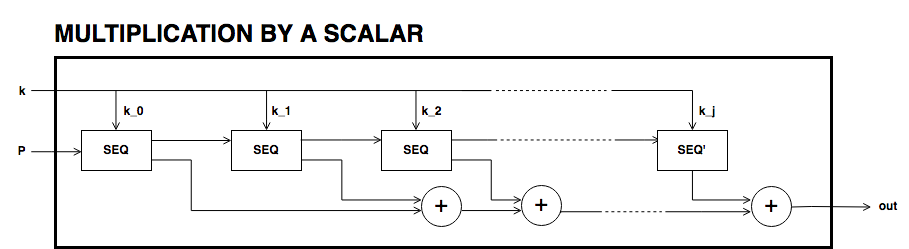
\includegraphics[scale=0.45]{Diag/Mult_by_scalar.png}
	\end{figure}
	
	\item Each \textsc{seq} box takes a point of $E$ of the from $P_i = 2^{248 i} P$ for $i=0,\dots,j-1$ and outputs two points %of $E$,
		$$ 	
			2^{248} \cdot P_i 
			\quad \text{and} \quad
			\sum_{n = 0}^{247} b_n \cdot 2^{n} \cdot P_i. 
		$$
	The first point is the input of the next $(i+1)$-th \textsc{seq} box (note that $ 2^{248} \cdot P_i = P_{i+1}$) whereas the second output is the computation of the $i$-th term in expression (\ref{kP}). The precise circuit is depicted in next two figures \textsc{seq} and \textsc{window}.
	
	\begin{figure}[h]
		\centering
		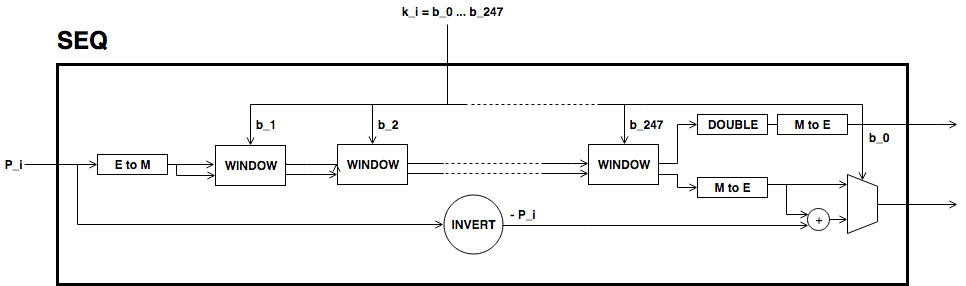
\includegraphics[scale=0.43]{Diag/Mult_by_scalar_SEQ.png}\\
		\vspace{0.5cm}
		
		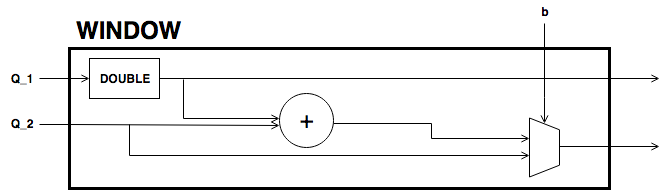
\includegraphics[scale=0.45]{Diag/Mult_by_scalar_SEQ_window.png}
		\vspace{0.3cm}
	\end{figure}

	The idea of the circuit is to first compute some point 		
		$$	Q = P_i + b_1 \cdot (2P_i) + b_2 \cdot (4P_i) 
				+ b_3 \cdot (8P_i) + \dots + b_{247} \cdot (2^{247}P_i), $$
	and output the point
		$$ Q - b_0 \cdot P_i. $$
	This permits the computation of $Q$ using the Montgomery form of Baby-Jubjub and only use twisted Edwards for the second calculation. The reason to change forms is that, in the calculation of the output, we may get a sum with input the point at infinity if $b_0 = 0$. 

	Still, we have to ensure that none of the points being doubled or added when working in $E_M$ is the point at infinity and that we never add the same two points. 

	\begin{itemize}
		
		% None of the points being doubled is the point at infinity.
		\item By assumption, $P\not= O$ and ord$(P)>8$. Hence, by Lagrange theorem {\cite[Corollary 4.12]{lagrange}}, $P$ must have order $r$, $2r$, $4r$ or $8r$. 
		For this reason, none of the points in $E_M$ being doubled or added in the circuit is the point at infinity, because for any integer $m$,  $2^m$ is never a multiple of $r$, even when $2^m$ is larger than $r$, as $r$ is a prime number. Hence, $2^m \cdot P \not= O$ for any $m\in\Z$.		

		% Addition: different points.
		\item Looking closely at the two inputs of the sum, it is easy to realize that they have different parity, one is an even multiple of $P_i$ and the other an odd multiple of $P_i$, so they must be different points. Hence, the sum in $E_M$ is done correctly.
	\end{itemize}
	
	\item The last term of expression (\ref{kP}) is computed in a very similar manner. The difference is that the number of bits composing $k_j$ may be shorter and that there is no need to compute $P_{j+1}$, as there is no other \textsc{seq} box after this one. So, there is only output, the point $k_j \cdot P_j = k_j\cdot 2^{248j} P$. This circuit is named \textsc{seq'}.
	
	\begin{figure}[h]
		\centering
		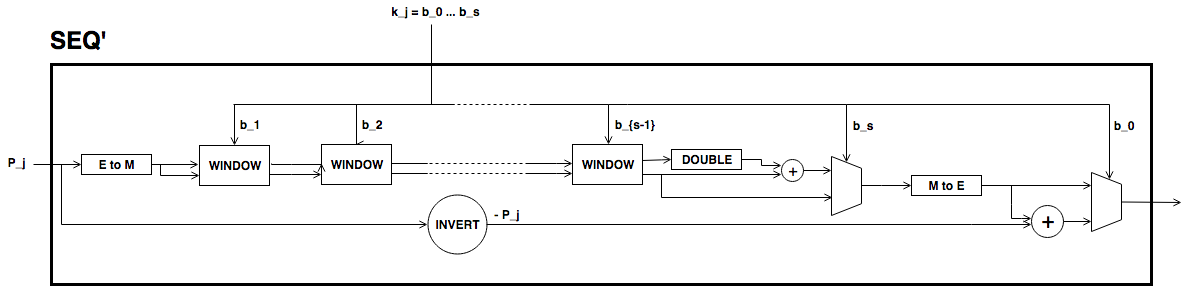
\includegraphics[scale=0.43]{Diag/Mult_by_scalar_SEQ_prime.png}
	\end{figure}
	
\end{enumerate}


\section {Pedersen hash}			 			% !TEX root =/home/marta/Dropbox/Documents/Especificacions/Pedersen/Description.tex

Let $M$ be a sequence of bits. We construct the Pedersen hash of $M$ as follows:
% We construct the Pedersen hash as follows: 
\begin{itemize}
	\item Sample $P_0,P_1,\dots,P_k$ uniformly in $\G$ (for some specified integer $k$). %Cal que k geq l.
	%, in our case $k=5$).
	%	Let $P_0,P_1,\dots,P_k$ be uniformly sampled generators of $\G$. 
	% These points only need to be computed once.
	% First, we sample elements (generators) $P_0,P_1,\dots,P_k$ uniformly in $\G$ (for some specified integer $k$, in our case $k=5$). 
	% En el codi de Jordi: allò de typeof?
	\item   Split $M$ into sequences of 4 bits{\footnote{If $M$ is not a multiple of 4, pad $M$ to a multiple of 4 bits by appending zero bits.}}. 
	More precisely, write  
	\begin{gather*}
		M = M_1M_2\dots M_l 
		\quad\text{where}\quad
		M_i = m_1m_2\dots m_{k_i}
		\quad\text{with}\quad 
		\begin{cases}
			k_i = 50 	\;\text{ for }  i = 0, \dots, l-1, \\
			k_l \leq 50,
		\end{cases}
	\end{gather*}
	where the $m_j$ terms are 4-bit chunks $[b_0^j\: b_1^j\: b_2^j\: b_3^j]$. 
	Define  
	$$ enc(m_j) = (2b_3^j-1) 
		\cdot (1+b_{0}^j+2b_{1}^j+4b^j_{2}) $$
	and let 
	$$ \langle M_i \rangle = \sum_{j=1}^{k_i} enc(m_j) \cdot 2^{5(j-1)}.	$$
	We define the Pedersen hash of $M$ as
	\begin{equation}
	\label{eq-ped}
		H(M) = \langle M_0 \rangle \cdot P_0 
		+  \langle M_1 \rangle \cdot P_1 
		+  \langle M_2 \rangle \cdot P_2 
		+ \dots + \langle M_l \rangle \cdot P_l.	
	\end{equation}
	Note that the expression above is a linear combination of elements of $\G$, 
	so itself is also an element of $\G$. 
	That is, the resulting Pedersen hash $H(M)$ is a point of the elliptic curve $E$ of order $r$.
\end{itemize}

The computation of the Pedersen hash has two steps: first, the base points $P_0, P_1, \dots, P_k$ need to be generated. This only needs to be done once, as they can be reused to compute hashes of other data. And secondly, the calculation of expression (\ref{eq-ped}). The circuits used to compute this sum are quite similar to the ones used to calculate the multiple of a point of an elliptic curve except that here we only work with the twisted Edwards form of $E$ and we can have many points precalculated, so instead of doubling all the time, we work with look-up tables. 
\label{sec-ped}
	\subsection{Set of generators} 				%%
{\color{blue}{Barry!}}
%%
We generate the points $P_0,\dots,P_k$ described in section \ref{sec-ped} in such a manner that it is difficult to find a connection between any of these two points. 
More precisely, we take 
	\texttt{D =  "Iden3$\_$PedersenGenerator$\_$"} 
followed by a byte 
	\texttt{S} 
holding that smallest number that 
	\texttt{H = Blake2s-256(D || S)} 
results in a point in the elliptic curve. We use the specification of Blake2s-256 hash function defined in
	\url{https://tools.ietf.org/html/rfc7693#appendix-D}.

% TODO: Add what happens if $g_i = k \times g_{i+1}$? Show it is easy to invert the hash function?
	\subsection{Computation} 					In \textsc{pedersen hash}, we have depicted the circuit used to compute (equatio \ref{eq-ped}). Each \textsc{multiplication} box returns one term of the sum. 

%that takes, per bit, that many constraints (of a circuit). 

\begin{figure}[h]
	\centering
	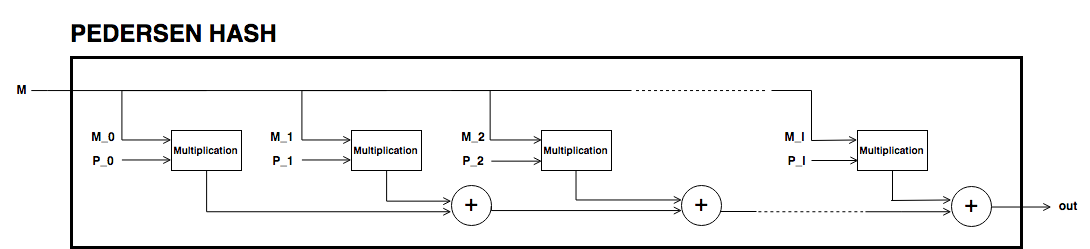
\includegraphics[scale=0.4]{Diag/Ped_Hash.png}
	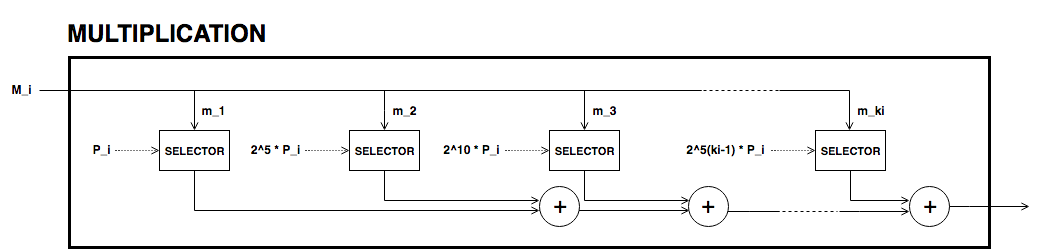
\includegraphics[scale=0.4]{Diag/Ped_Hash_Multiplication.png}
\end{figure}

As the set of generators are fixed, we can precompute its multiples and use 4-bit lookup windows to select the right points. This is done as shown in next circuit \textsc{selector}.

\begin{figure}[h]
	\centering
	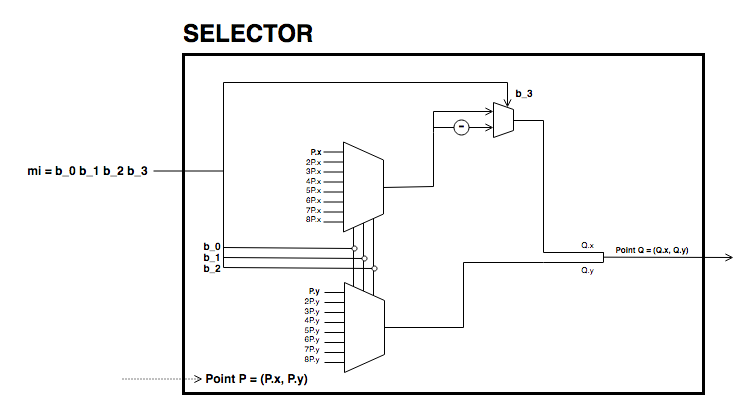
\includegraphics[scale=0.5]{Diag/Ped_Hash_Multiplication_selector.png}
\end{figure}

The circuit receives as input a 4-bit chunk. The first three bits are used to select the right multiple of the point and last bit decides the sign of the point. Recall that negation on a point of a twisted Edwards curve corresponds to negation of its first coordinate. 

%
%
%{\bf{Diagram}}	\\\vspace{-0.3cm}				%\input{Mult-diagram}
%
%Let $G$ be one of the generators. Consider a 4-bit window \fbox{$s_0$}\fbox{$s_1$}\fbox{$s_2$}\fbox{$s_3$} . Bit $s_3$ is used to determine the sign and $s_0, s_1, s_2$ the point. \\
%
%
%
%
	
	\subsection{There is no overflow}	 		% !TEX root =/home/marta/Dropbox/Documents/Especificacions/Pedersen/Description.tex

We have seen we use a windowed scalar multiplication algorithm with signed digits. Each 4-bit message chunk corresponds to a window called \textsc{selector} and each chunk is encoded as an integer from the set $\{-8..8\}\backslash \{0\}$. 
% and we allow to have up to $50$ windows. 
This allows a more efficient lookup of the window entry for each chunk than if the set $\{1..16\}$ had been used, because a point can be conditionally negated using only a single constraint \cite{sapling}.\\
% Sapling, the new network upgrade of Zcash, uses 3-bit windows but we propose to use 4-bit windows, as it requires less constraints per bit.\\




As we have up to 50 segments per each generator $P_i$, the largest multiple of the generator $P_i$ is $n\cdot P_i$ with 
$$n = 2^0 \times8 + 2^5 \times 8 + \left(2^5\right)^2 \times8 \dots + 	2^{245}\times 8 .$$
We have to make sure that this number is smaller than $(r-1)/2$, where $r$ is the order of the large prime subgroup of the curve.  Indeed,
\begin{align*}
	\quad\; n 
	& = 8 \times \sum_{ k = 0}^{49} 2^{5k}
	= 8 \times \frac{2^{250}-1}{2^5-1}\\
	& = 466903585634339497675689455680193176827701551071131306610716064548036813064%\\
\end{align*}
\vspace{-0.2cm}
and 
%
\begin{align*}
	\frac{r-1}{2} &= 1368015179489954701390400359078579693038406986079283629600107830474223686520 \\
	& > n.\\ \vspace{0.4cm}
\end{align*}

%\input{Mult-constraints}
	\subsection{Number of constraints per bit}	% !TEX root =/home/marta/Dropbox/Documents/Especificacions/Pedersen/Description.tex

%%

% Consider 3-bit lookup windows \fbox{$s_0$}\fbox{$s_1$}\fbox{$s_2$} and 4-lookup windows \fbox{$s_0$}\fbox{$s_1$}\fbox{$s_2$}\fbox{$s_3$}.\\

When using 3-bit and 4-bit windows, we have {{\bf 1 constraint for the sign}} and {{\bf 3 for the sum}} (as we are using the Montgomery form of the curve, that requires only 3). Now let's look at the constraints required for the multiplexers. \\

With 3-bit windows we need only one constraint per multiplexer, so {\bf 2 constraints} in total. \\

Standard 4-bit windows require two constraints: one for the output and another to compute $s_0*s_1$. So, a priori we would need 4 constraints, two per multiplexer. But we can reduce it to 3 as the computation of $s_0*s_1$ is the same in both multiplexers, so this constraint can be reused. This way only {{\bf 3 constraints}} are required. \\

So, the amount of constraints per bit are:
\begin{itemize}
	\item 3-lookup window : %\fbox{$s_0$}\fbox{$s_1$}\fbox{$s_2$} : 
		$ (1+3+2)/3 = 2 $ constraints per bit.
	\item 4-lookup window : %\fbox{$s_0$}\fbox{$s_1$}\fbox{$s_2$}\fbox{$s_3$} : 
		$ (1 +3+3)/4 = 1.75 $ constraints per bit. 
\end{itemize}

The specific constraints can be determined as follows: let the multiplexers of coordinates x and y be represented by the following look up tables:
%The specific constraints are the following ones. Let the multiplexers of the coordinates $x$ and $y$ be represented by the following look up tables:
%
%%
\begin{table}[h]
    \begin{minipage}{.5\linewidth}
      \centering
	\begin{tabular}{c|c|c|c}
                $s_2$ & $s_1$ & $s_0$ & $out$\\
                	\hline
                	0 & 0 & 0 & $a_0$\\
                	0 & 0 & 1 & $a_1$\\
                	0 & 1 & 0 & $a_2$\\
                	0 & 1 & 1 & $a_3$\\
                	1 & 0 & 0 & $a_4$\\
                	1 & 0 & 1 & $a_5$\\
                	1 & 1 & 0 & $a_6$\\
                	1 & 1 & 1 & $a_7$
      	\end{tabular}
    \end{minipage}%
    \begin{minipage}{.5\linewidth}
      \centering
	\begin{tabular}{c|c|c|c}
		$s_2$ & $s_1$ & $s_0$ & $out$\\
		\hline
		0 & 0 & 0 & $b_0$\\
		0 & 0 & 1 & $b_1$\\
		0 & 1 & 0 & $b_2$\\
		0 & 1 & 1 & $b_3$\\
		1 & 0 & 0 & $b_4$\\
		1 & 0 & 1 & $b_5$\\
		1 & 1 & 0 & $b_6$\\
		1 & 1 & 1 & $b_7$
	\end{tabular}
    \end{minipage} 
\end{table}

\noi We can express them with the following 3 constraints:
% Then, we can express both multiplexers using the following 3 constraints:
%%
\begin{itemize}
    \item 	$aux = s_0 s_1$ %(Reused for both multiplexers)
    \item 	$out = [ (a_7-a_6-a_5+a_4-a_3+a_2+a_1-a_0)*aux 
    		+ (a_6-a_4-a_2+a_0)*s_1$ \\
    		$\text{\qquad\;\;} + (a_5-a_4-a_1+a_0)*s_0
    		+ (a_4 - a_0) ] z 
    		+ (a_3-a_2-a_1+a_0)*aux + (a_2-a_0)*s_1 + (a_1-a_0)*s_0+ a_0$
    \item	$ out = [ (b_7-b_6-b_5+b_4-b_3+b_2+b_1-b_0)*aux 
    		+ (b_6-b_4-b_2+b_0)*s_1$ \\
    		$\text{\qquad\;\;} + (b_5-b_4-b_1+b_0)*s_0 
    		+ (b_4 - b_0)] z 
    		+ (b_3-b_2-b_1+b_0)*aux + (b_2-b_0)*s_1 + (b_1-b_0)*s_0+ b_0$\\
\end{itemize}
%%
		

%TODO: Important! El tema del bit del signe? Zero o tres?
{\color{blue}{Es bo o b3? El tema del bit del signe!}}  \item 

\newpage
\addcontentsline{toc}{section}{References}
\bibliographystyle{acm}
\bibliography{lit}

\end{spacing}
\end{document}